\documentclass{ctexart}
\usepackage{amsmath}
\usepackage{geometry}
\usepackage{graphicx}
\geometry{a4paper, margin=1in}

\begin{document}

\section{直方图均衡化在灰度集中的图像中的失真分析}

直方图均衡化(Histogram Equalization, HE)是一种常见的图像增强方法,其基本思想是通过灰度级的变换,使得输出图像的灰度分布尽可能接近均匀分布,从而提升图像对比度。设一幅灰度图像的像素灰度值为离散变量 $r \in \{0, 1, 2, \dots, L-1\}$,其中 $L$ 通常取 256。图像的归一化灰度直方图可表示为 $p_r(r_k) = \frac{n_k}{n}$,其中 $n_k$ 表示灰度值为 $r_k$ 的像素个数,$n$ 为图像总像素数,$p_r(r_k)$ 表示灰度为 $r_k$ 的像素出现的概率。HE 所采用的映射函数基于输入图像的累积分布函数(CDF),定义为
\[
s_k = T(r_k) = (L - 1) \cdot \sum_{j=0}^{k} p_r(r_j),
\]
其中 $s_k$ 为变换后的灰度值,$T(r_k)$ 为映射函数,其本质上是对原始概率密度函数的积分。

该变换函数具有单调递增、非线性的特点,能够将输入图像的灰度分布拉伸至更广泛的范围。然而,当图像的灰度分布高度集中时,HE 方法会出现严重的问题。例如,设图像中几乎所有像素的灰度值集中在 $[0,10]$ 区间,而其它灰度值几乎没有像素占据。此时,直方图在低灰度区域聚集,累积分布函数在 $r_k > 10$ 时变化缓慢甚至趋于饱和,导致 $T(r_k)$ 在前 10 个灰度等级内迅速上升,而在其后的灰度区域趋于常数。这意味着原图中微小的灰度差异将被映射为输出图像中的大范围灰度差异,产生强烈的对比度拉伸。举一个极端的数学例子,设图像中只有两个灰度值:灰度为 0 的像素占 90\%,灰度为 1 的像素占 10\%。根据映射函数,可得
\[
T(0) = 255 \cdot 0.9 = 229.5, \quad T(1) = 255 \cdot (0.9 + 0.1) = 255。
\]
也就是说,原本仅有 1 个灰度单位的差异,在均衡化后被扩展为 25 个灰度单位以上。原本视觉上几乎不可分辨的黑与深灰,在处理后被强行拉伸为明亮灰与白,造成图像严重失真和不自然。

从数学上看,HE 的失真本质在于其映射函数 $T(r)$ 是基于全图灰度的累积分布,当图像灰度分布不均衡时(例如集中在暗区或亮区),变换函数将变得极度陡峭,导致微小的灰度差异被非线性放大。因此,虽然 HE 能在一定程度上提升对比度,但在灰度集中分布的图像中,其非线性拉伸作用可能导致伪影、过度增强和图像细节的损失,从而不适用于所有图像场景。
   \newpage
\section{实验}
   我们将使用 Python 语言实现直方图均衡化算法,并对其在灰度集中分布的图像中的失真进行分析。首先,我们生成一个灰度集中分布的图像,并对其进行直方图均衡化。然后,我们将其与原图进行比较,并分析其失真。
\begin{figure}[http]
        \centering
      
    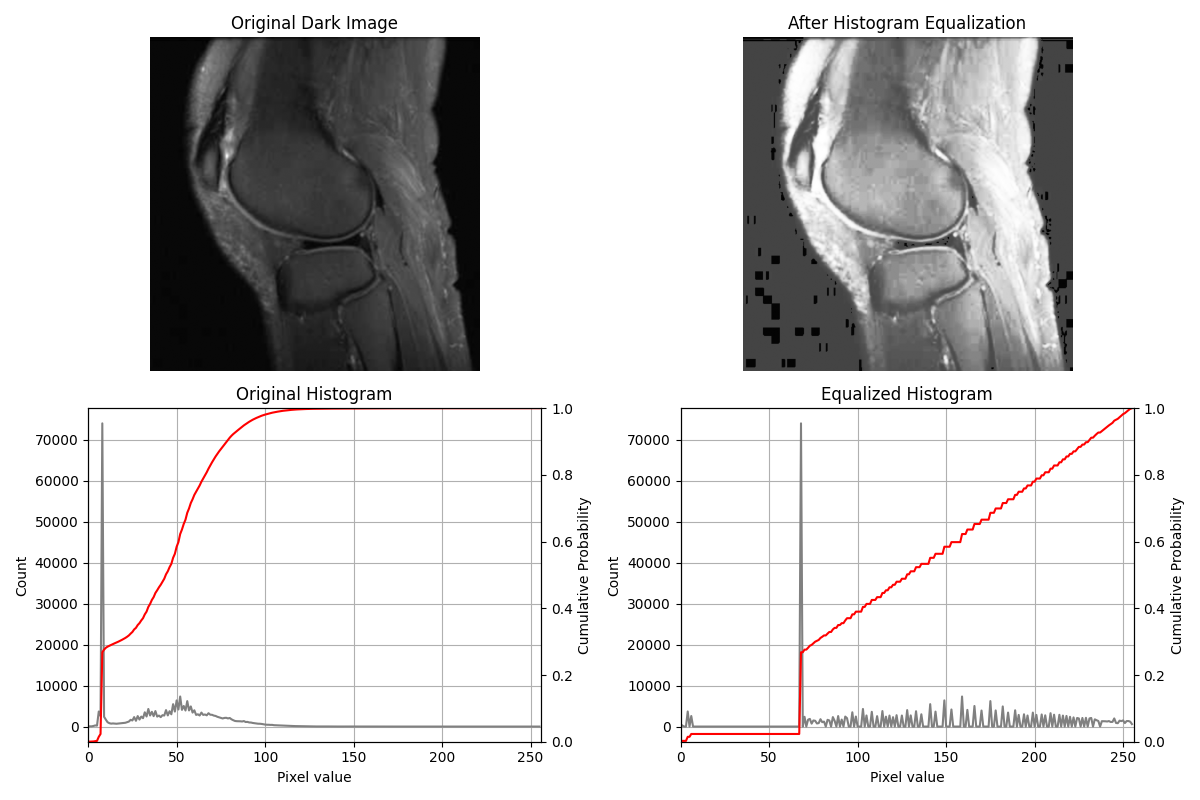
\includegraphics[width=0.8\textwidth]{Figure_1.png}
       \caption{Example of HE on a grayscale image}
    \end{figure}
   
显然,由于上图中的黑色区域十分之多,以灰度值在区间$[6,8]$的为例,大约有$80000$个,频数最多的灰度值为$8$累积概率达到了$26.82\%$,利用上一节的算式,可以得出\[T(8)=255\cdot 0.2682=68.04\]
在对其他区域进行类似的操作后,原本位于区间的像素点被均值化后变为了$[68,72]$,使上图中的大部分黑色的区域都被均衡化为灰白色,这就导致了图像的严重失真。


\end{document}
